\documentclass{article}
\usepackage{graphicx}
\usepackage{makecell}
\usepackage{listings}
\usepackage{geometry}
 \geometry{
 a4paper,
 total={174mm,261mm},
 left=18mm,
 top=18mm,
 }

\title{Network manual}
\author{Gabriele Pernici}
\date{December 2023}

\begin{document}

\maketitle

\section{Introduction}
This document contains the info on how to use the network program used in \textit{insert thesis name}. Section \ref{section:command} describes how to correctly generate a command file, in order to use the program. Section \ref{section:functionalities} describes in details how the program acts and the meaning of unclear parameters. Section \ref{section:files} describes the format of the files correlated to the program. More specifically the examples file, the network's structure Json file and the output file are described.
\\ \\ \\ \\
\begin{figure}[h]
    \label{img:diagram}
    \centering
    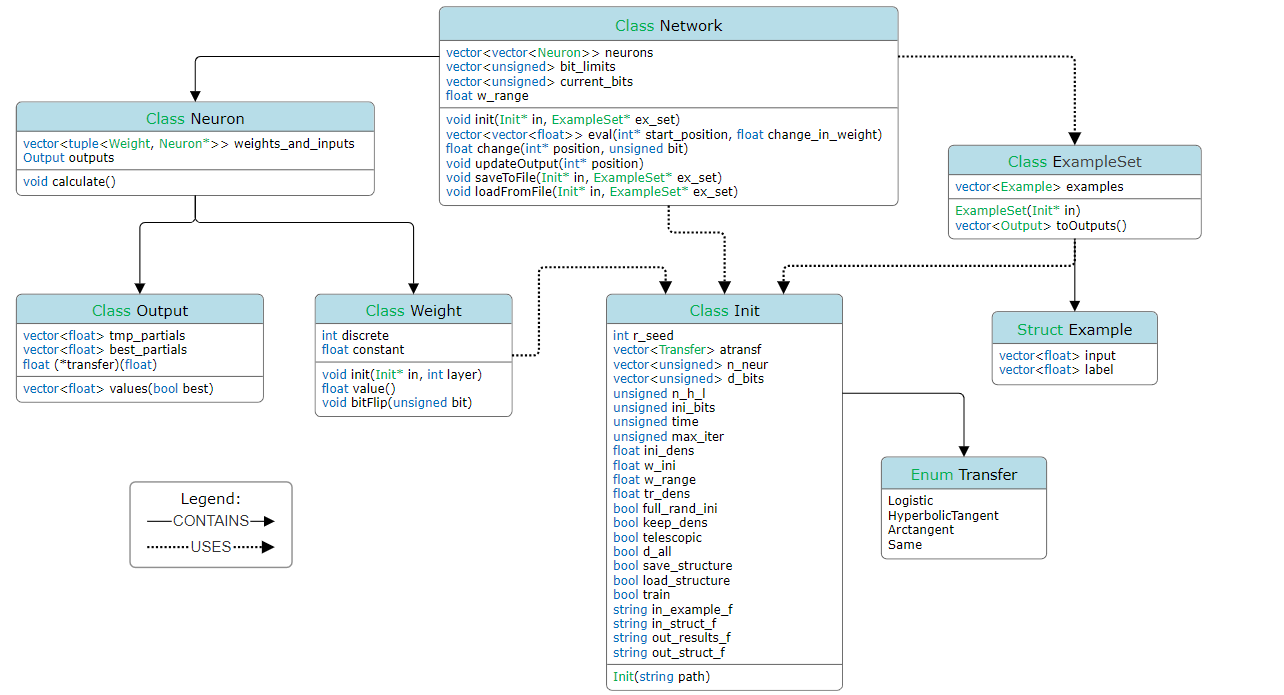
\includegraphics[width=1.0\textwidth]{NetworkStructure.PNG}
    \caption{This image shows the network's diagram of implementation.}
\end{figure}


\newpage
\section{Command file}\label{section:command}
The command file should be a text file (preferably with extension .cmd) with a combination of the following parameters. Each parameter, to be valid, has to be inserted as \textit{ParameterName ParameterValue1 ... ParameterValueN}. Each parameter should be on a different line of the file, however the order is not important. Every required parameter is in bald (if loading a network from file the only needed parameters are in italic) and every optional parameter has a default value. Moreover, for each parameter the number of values needed is stated. If a parameter has zero values required it means that the parameter name's presence is enough. Lastly, the type of value required is specified.
\begin{table}[h]
    \centering
    \begin{tabular}{|lccc|c|} 
        \hline
        \textbf{Name} & \textbf{nVal} & \textbf{Type} & \textbf{Def} & \textbf{Description}\\
        \hline
        r\_seed & 1 & N & 1 & \makecell{Random seed to generate the initial weights} \\\hline
        \textbf{n\_h\_l} & 1 & N & & \makecell{Number of hidden layers in the network} \\\hline
        \textbf{n\_neur} & n & N & & \makecell{Number of neuron per hidden layer} \\\hline
        atransf & n & {0,1,2} & 0 & \makecell{Type of transfer function of each layer. \\ Each number meaning is described in section \ref{section:functionalities}} \\\hline
        \textbf{d\_bits} & n & N & & \makecell{Max number of bits to use for discrete weights in each layer} \\\hline
        ini\_bits & 1 & N & d\_bits & \makecell{Number of bits to start discretization from} \\\hline
        time & 1 & N & $\infty$ & \makecell{Time limit for training} \\\hline
        max\_iter & 1 & N & $\infty$ & \makecell{Iterations limit for training} \\\hline
        ini\_dens & 1 & 0$<$x$<$1 & 1 & \makecell{Fraction of nonzero weight in the initialization phase} \\\hline
        w\_ini & 1 & x$>$0 & & \makecell{Weight range in initialization phase \\ compulsory if the full random parameter is absent} \\ \hline
        \textbf{w\_range} & 1 & x$>$0 & & \makecell{Weight range in training phase}  \\\hline
        tr\_dens & 1 & 0$<$x$<$1 & 1 & \makecell{Fraction of examples used in training} \\\hline
        full\_rand\_ini & 0 & & & \makecell{If present the program initializes \\ all weight values completely randomly \\ otherwise the w\_ini parameter is used} \\\hline
        keep\_dens & 0 & & & \makecell{If present the program tries to keep \\ the value of ini\_dens during training} \\\hline
        telescopic & 0 & & & \makecell{If present the program uses \\ the telescopic mode during training} \\\hline
        d\_all & 0 & & & \makecell{If present the program looks for the best \\ improving move during training} \\\hline
        save & 0 & & & \makecell{If present the program saves \\ the network's structure after training} \\\hline
        \textit{load} & 0 & & & \makecell{If present the program loads \\ the netowrk structure from in\_struct\_f} \\\hline
        train & 0 & & & \makecell{If present the program trains \\ the network, otherwise it's evaluated} \\\hline
        \textbf{\textit{in\_example\_f}} & 1 & String & & \makecell{Path of the examples file. Always needed} \\\hline
        \textit{in\_struct\_f} & 1 & String & & \makecell{Path of the network's structure file} \\\hline
        out\_results\_f & 1 & String & ./out.exa & \makecell{Path where the results are saved} \\\hline
        out\_struct\_f & 1 & String & ./net.json & \makecell{Path where the network's structure is saved} \\
        \hline
    \end{tabular}
\end{table}


\newpage
\section{Program functionalities}\label{section:functionalities}

\subsection{Transfer functions details}
As stated in the previous section, the \textbf{\textit{atransf}} parameter can assume 3 values that each represent a different type of transfer function. 0 represents the standard logistic function, 1 represents the symmetric logistic function (aka the hyperbolic tangent) and 2 represents the arctangent function.

\subsection{Program operations}
The program's main functionalities are to train or evaluate the specified network. The \textbf{\textit{train}} parameter in the command file specifies which of the two the program will do. 

Moreover, the program can save the network's structure after the end of the main operations, using the \textbf{\textit{save}} parameter. This is fundamental in order to save the weights achieved during training, or to stop (using the iterations or the time limit) a training process and continue it later, without having to start from scratch.

Lastly, the program can load a previously saved network in order to evaluate, or keep training it, by using the \textbf{\textit{load}} parameter. When doing so the program file is greatly shortened as the only needed parameters are: \textit{load, in\_example\_f, in\_struct\_f}. The following parameters are optional and their value, if not present, will be set either accordingly to the json file (where present) or as their default: \textit{d\_bits, ini\_bits, time, max\_iter, tr\_dens, save, train, telescopic, d\_all, keep\_dens, out\_results\_f, out\_struct\_f}. All other parameters are useless and, if present, will be ignored.

Any combination of the \textit{train, save, load} parameters is accepted.


\section{Files}\label{section:files}

\subsection{Sample/Output file}
The suggested filename extension is .exa. In some cases, output values are
not used (e.g., when evaluating a trained network). In such case, they can be
set to zero.
Files containing the examples or the outputs have the following format:
\\
\begin{table}[h]
    \centering
    \begin{tabular}{l}
        \hline
        n\_inp $n_{inputs}$ \\
        n\_out $n_{outputs}$ \\
        n\_patt $n_{patterns}$ \\
        pattern $x_1$ \quad $x_2$ \quad \ldots \quad $x_{n_{inputs}}$ \quad $y_1$ \quad $y_2$ \quad \ldots \quad $y_{n_{outputs}}$ \\
        \ldots \\
        pattern $x_1$ \quad $x_2$ \quad \ldots \quad $x_{n_{inputs}}$ \quad $y_1$ \quad $y_2$ \quad \ldots \quad $y_{n_{outputs}}$ \\
        \hline
   \end{tabular}
\end{table}  

\newpage
\subsection{Network structure file}
The following is the format of the network's structure json file. The first layer of neurons is not saved (as can be seen by the first "pos" parameter) as it is used to represent the input examples, so it's useless to save. In the file are saved the info regarding the network's structure.
\begin{lstlisting}[escapechar=|]

{
    "neurons": [
        {
            "pos":[1,0],
            "weights": [
                {
                    "index":0,
                    "discrete":|\textit{value}|,
                    "constant":|\textit{value}|
                },
                
                ...
                
                {
                    "index":n,
                    "discrete":|\textit{value}|,
                    "constant":|\textit{value}|
                }
            ]
        },

        ...
        
        {
            "pos":[x,y],
            "weights": [
                {
                    "index":0,
                    "discrete":|\textit{value}|,
                    "constant":|\textit{value}|
                },

                ...
                
                {
                    "index":n,
                    "discrete":|\textit{value}|,
                    "constant":|\textit{value}|
                }
            ]
        }
    ],
    "bit_limits": [|\textit{values}|],
    "current_bits": [|\textit{values}|],
    "w_range":|\textit{value}|,
    "atransf":[|\textit{values}|],
}
\end{lstlisting}

\end{document}
